\subsection{TWS}
\label{subsec:tws}
\begin{tcoloritemize}
    \blueitem{TWS}{
    \textbf{T}rack \textbf{W}hile \textbf{S}can --- reference \cref{fig:sensors_aa:apg68:tws:search} for symbology

    \begin{subitemize}
        \item \textbf{Multi-target tracking mode}
        \begin{itemize}
            \item Allows multi-target AIM-120 engagement
            \item Targets not locked --- \textbf{\underline{no RWR warning}}
        \end{itemize}
        \item \textbf{FCR builds trackfiles for each target}
        \begin{itemize}
            \item Predicts target movement between scans
            \item Slow update rate --- target maneuvers can cause radar to lose track
        \end{itemize}
        \item \textbf{Trackfiles can be in several states}
        \begin{itemize}
            \item Search / Track / System / Cursor / Bugged
        \end{itemize}
        \textbf{Reference \cref{subsec:sensorsaa:apg68:tws:trackfile} \& \cref{fig:sensorsaa:apg68:tws:trackfile} for trackfile symbology}
    \end{subitemize}}
\end{tcoloritemize}

\begin{figure}[htbp]
    \centering
    \begin{tikzpicture}[auto, node distance=10mm, x=1mm, y=1mm, very thick, line cap=round,
        >={Latex[round]}
        ]
        
        \node[] (mfd) at (0,0) {
            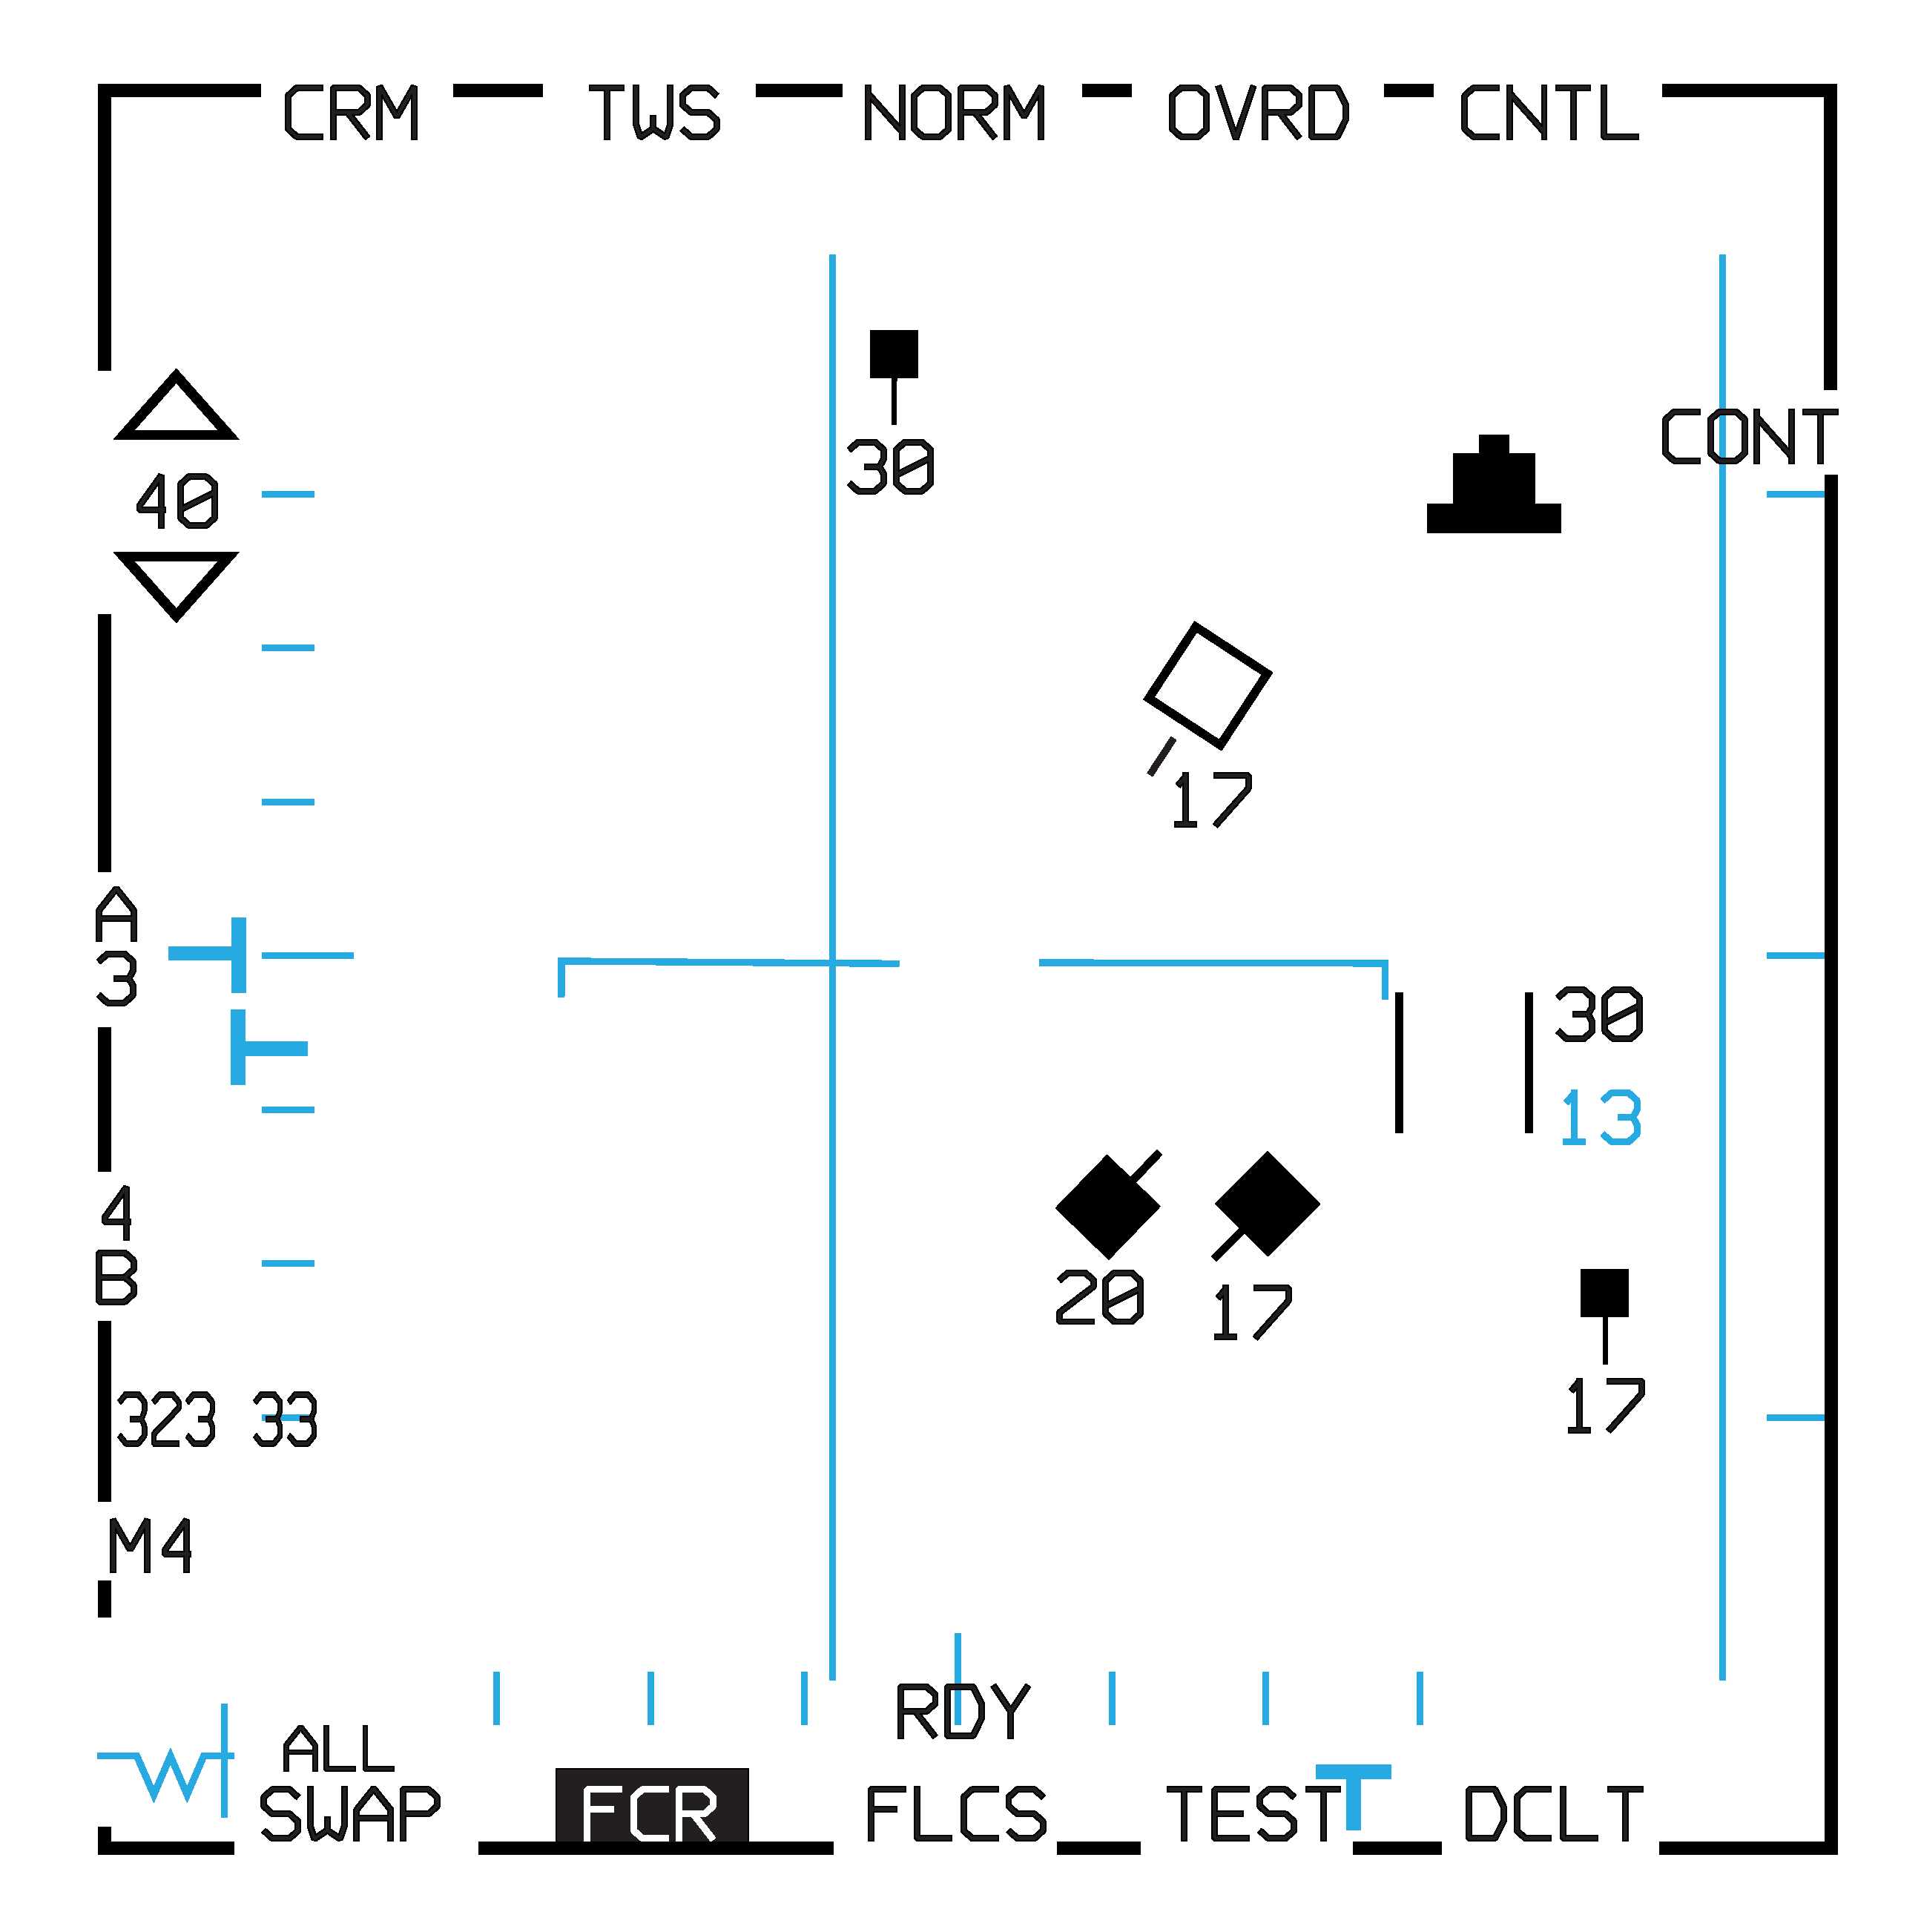
\includegraphics[
                height=75mm,
            ]{mfd/fcr_aa/tws_search.pdf}
        };

        % Annotations
        \node[lannot] (search) at ($(fig.west)+(0mm,28mm)$) {Search target};
        \draw[->, red] (search.east) -- ++(30mm, 0mm) -- ++(4mm, -4mm);

        \node[lannot] (sec) at ($(fig.west)+(0mm,8mm)$) {Azimuth scan limits};
        \draw[->, red] (sec.east) -- ++(32mm, 0mm);

        \node[rannot] (as) at ($(fig.east)+(0mm,24mm)$) {Current STPT};
        \draw[->, red] (as.west) -- ++(-12mm, 0mm) -- ++(-3mm, -3mm);

        \node[rannot] (system) at ($(fig.east)+(0mm,10mm)$) {System \\ target};
        \draw[->, red] (system.west) -- ++(-26mm, 0mm);

        \node[rannot] (cursor) at ($(fig.east)+(0mm,-4mm)$) {Acquisition cursor};
        \draw[->, red] (cursor.west) -- ++(-11mm, 0mm);

        \node[rannot] (searchr) at ($(fig.east)+(0mm,-15mm)$) {Search \\ target};
        \draw[->, red] (searchr.west) -- ++(-11mm, 0mm);

        \node[rannot] (asec) at ($(fig.east)+(0mm,-26mm)$) {Track \\ targets};
        \draw[->, red] (asec.west) -- ++(-20mm, 0mm) -- ++(-6mm,10mm);
    \end{tikzpicture}
    \caption{Basic TWS search FCR page symbology.}
    \label{fig:sensors_aa:apg68:tws:search}
\end{figure}

\begin{figure}[htbp]
    \centering
    \begin{subfigure}[b]{0.15\linewidth}
        \centering
        
\includegraphics[
            scale=0.75,
        ]{mfd/fcr_aa/tgt_search.pdf}
        \caption{Search}
        \label{fig:sensorsaa:apg68:tws:trackfile:search}
    \end{subfigure}
    \begin{subfigure}[b]{0.15\linewidth}
        \centering
        
\includegraphics[
            scale=0.75,
        ]{mfd/fcr_aa/tgt_track.pdf}
        \caption{Track}
        \label{fig:sensorsaa:apg68:tws:trackfile:track}
    \end{subfigure}
    \begin{subfigure}[b]{0.15\linewidth}
        \centering
        
\includegraphics[
            scale=0.75,
        ]{mfd/fcr_aa/tgt_system.pdf}
        \caption{System}
        \label{fig:sensorsaa:apg68:tws:trackfile:system}
    \end{subfigure}
    \begin{subfigure}[b]{0.15\linewidth}
        \centering
        
\includegraphics[
            scale=0.75,
        ]{mfd/fcr_aa/tgt_cursor.pdf}
        \caption{Cursor}
        \label{fig:sensorsaa:apg68:tws:trackfile:cursor}
    \end{subfigure}
    \begin{subfigure}[b]{0.15\linewidth}
        \centering
        
\includegraphics[
            scale=0.75,
        ]{mfd/fcr_aa/tgt_bugged.pdf}
        \caption{Bugged}
        \label{fig:sensorsaa:apg68:tws:trackfile:bugged}
    \end{subfigure}
    \caption{TWS Track Symbols}
    \label{fig:sensorsaa:apg68:tws:trackfile}
\end{figure}

\subsubsection{TRACKFILE STATES}
\label{subsec:sensorsaa:apg68:tws:trackfile}
\begin{tcoloritemize}
    \blueitem{Search Target}{
    \begin{subitemize}
        \item \textbf{Initial state for radar returns}
        \begin{itemize}
            \item Not enough information to generate track
            \item Automatic transition to track after 1-2 radar sweeps
        \end{itemize}
        \item \textbf{Display} --- similar to RWS radar brick
        \item \textbf{Reference \cref{fig:sensorsaa:apg68:tws:trackfile:search}}
    \end{subitemize}}
    \blueitem{Track Target}{
    \begin{subitemize}
        \item \textbf{FCR automatically correlates radar return data to form track files}
        \begin{itemize}
            \item Tracks target velocity, angle, altitude etc.
            \item \textbf{\underline{Maximum of 10 trackfiles}}, lowest priority dropped if exceeded
        \end{itemize}
        \item \textbf{Can be manually transitioned to higher modes by pilot to prioritize}
        \item \textbf{Reference \cref{fig:sensorsaa:apg68:tws:trackfile:track}}
    \end{subitemize}}
    \blueitem{System Target}{
    \begin{subitemize}
        \item \textbf{Allows pilot to designate targets of interest}
        \begin{itemize}
            \item For monitoring
            \item For future weapons employment
        \end{itemize}
        \item \textbf{No additional radar energy allocated to System Targets}
        \item \textbf{Reference \cref{fig:sensorsaa:apg68:tws:trackfile:system}}
    \end{subitemize}}
    \blueitem{Cursor Target}{
    \begin{subitemize}
        \item \textbf{Acquisition Cursor ``snaps'' to nearby System Targets} --- therefore named Cursor Targets
        \item \textbf{Scan centered on Cursor Target}
        \begin{itemize}
            \item 3 bar elevation
            \item $\pm$25 deg azimuth pattern 
            \item Reduces chance of losing track
        \end{itemize}
        \item \textbf{Reference \cref{fig:sensorsaa:apg68:tws:trackfile:cursor,fig:sensorsaa:apg68:tws:cursorsymb}}
    \end{subitemize}}
    \blueitem{Bugged Target}{
    \begin{subitemize}
        \item \textbf{Selected for weapons employment}
        \begin{itemize}
            \item Can guide AIM-120C (w/o STT Lock)
            \item DLZ displayed if missile selected
            \item Launched AIM-120 will continue to guide even if another target is bugged --- \textbf{\underline{allows for multi-target engagement}}
        \end{itemize}
        \item \textbf{Scan Centered on Bugged Target}
        \begin{itemize}
            \item 3 bar elevation
            \item $\pm$25 deg azimuth pattern 
            \item Reduces chance of losing track
        \end{itemize}
        \item \textbf{TMS Right --- Cycles through System Targets in range order} (bugs closest if none bugged)
        \item \textbf{Reference \cref{fig:sensorsaa:apg68:tws:trackfile:bugged,fig:sensorsaa:apg68:tws:buggedsymb}}
    \end{subitemize}}
    \blueitem{Spotlight}{
    \begin{subitemize}
        \item \textbf{Narrow scan centered on acquisition cursor}
        \begin{itemize}
            \item 4 bar elevation 
            \item \pm10 deg azimuth
        \end{itemize}
        \item \textbf{Allows pilot to override TWS scan priority}
        \item \textbf{Activated by holding TMS Forward >1 sec}
    \end{subitemize}}
\end{tcoloritemize}

\begin{figure}[htbp]
    \centering
    \begin{tikzpicture}[auto, node distance=10mm, x=1mm, y=1mm, very thick, line cap=round,
        >={Latex[round]}
        ]
        
        \node[] (mfd) at (0,0) {
            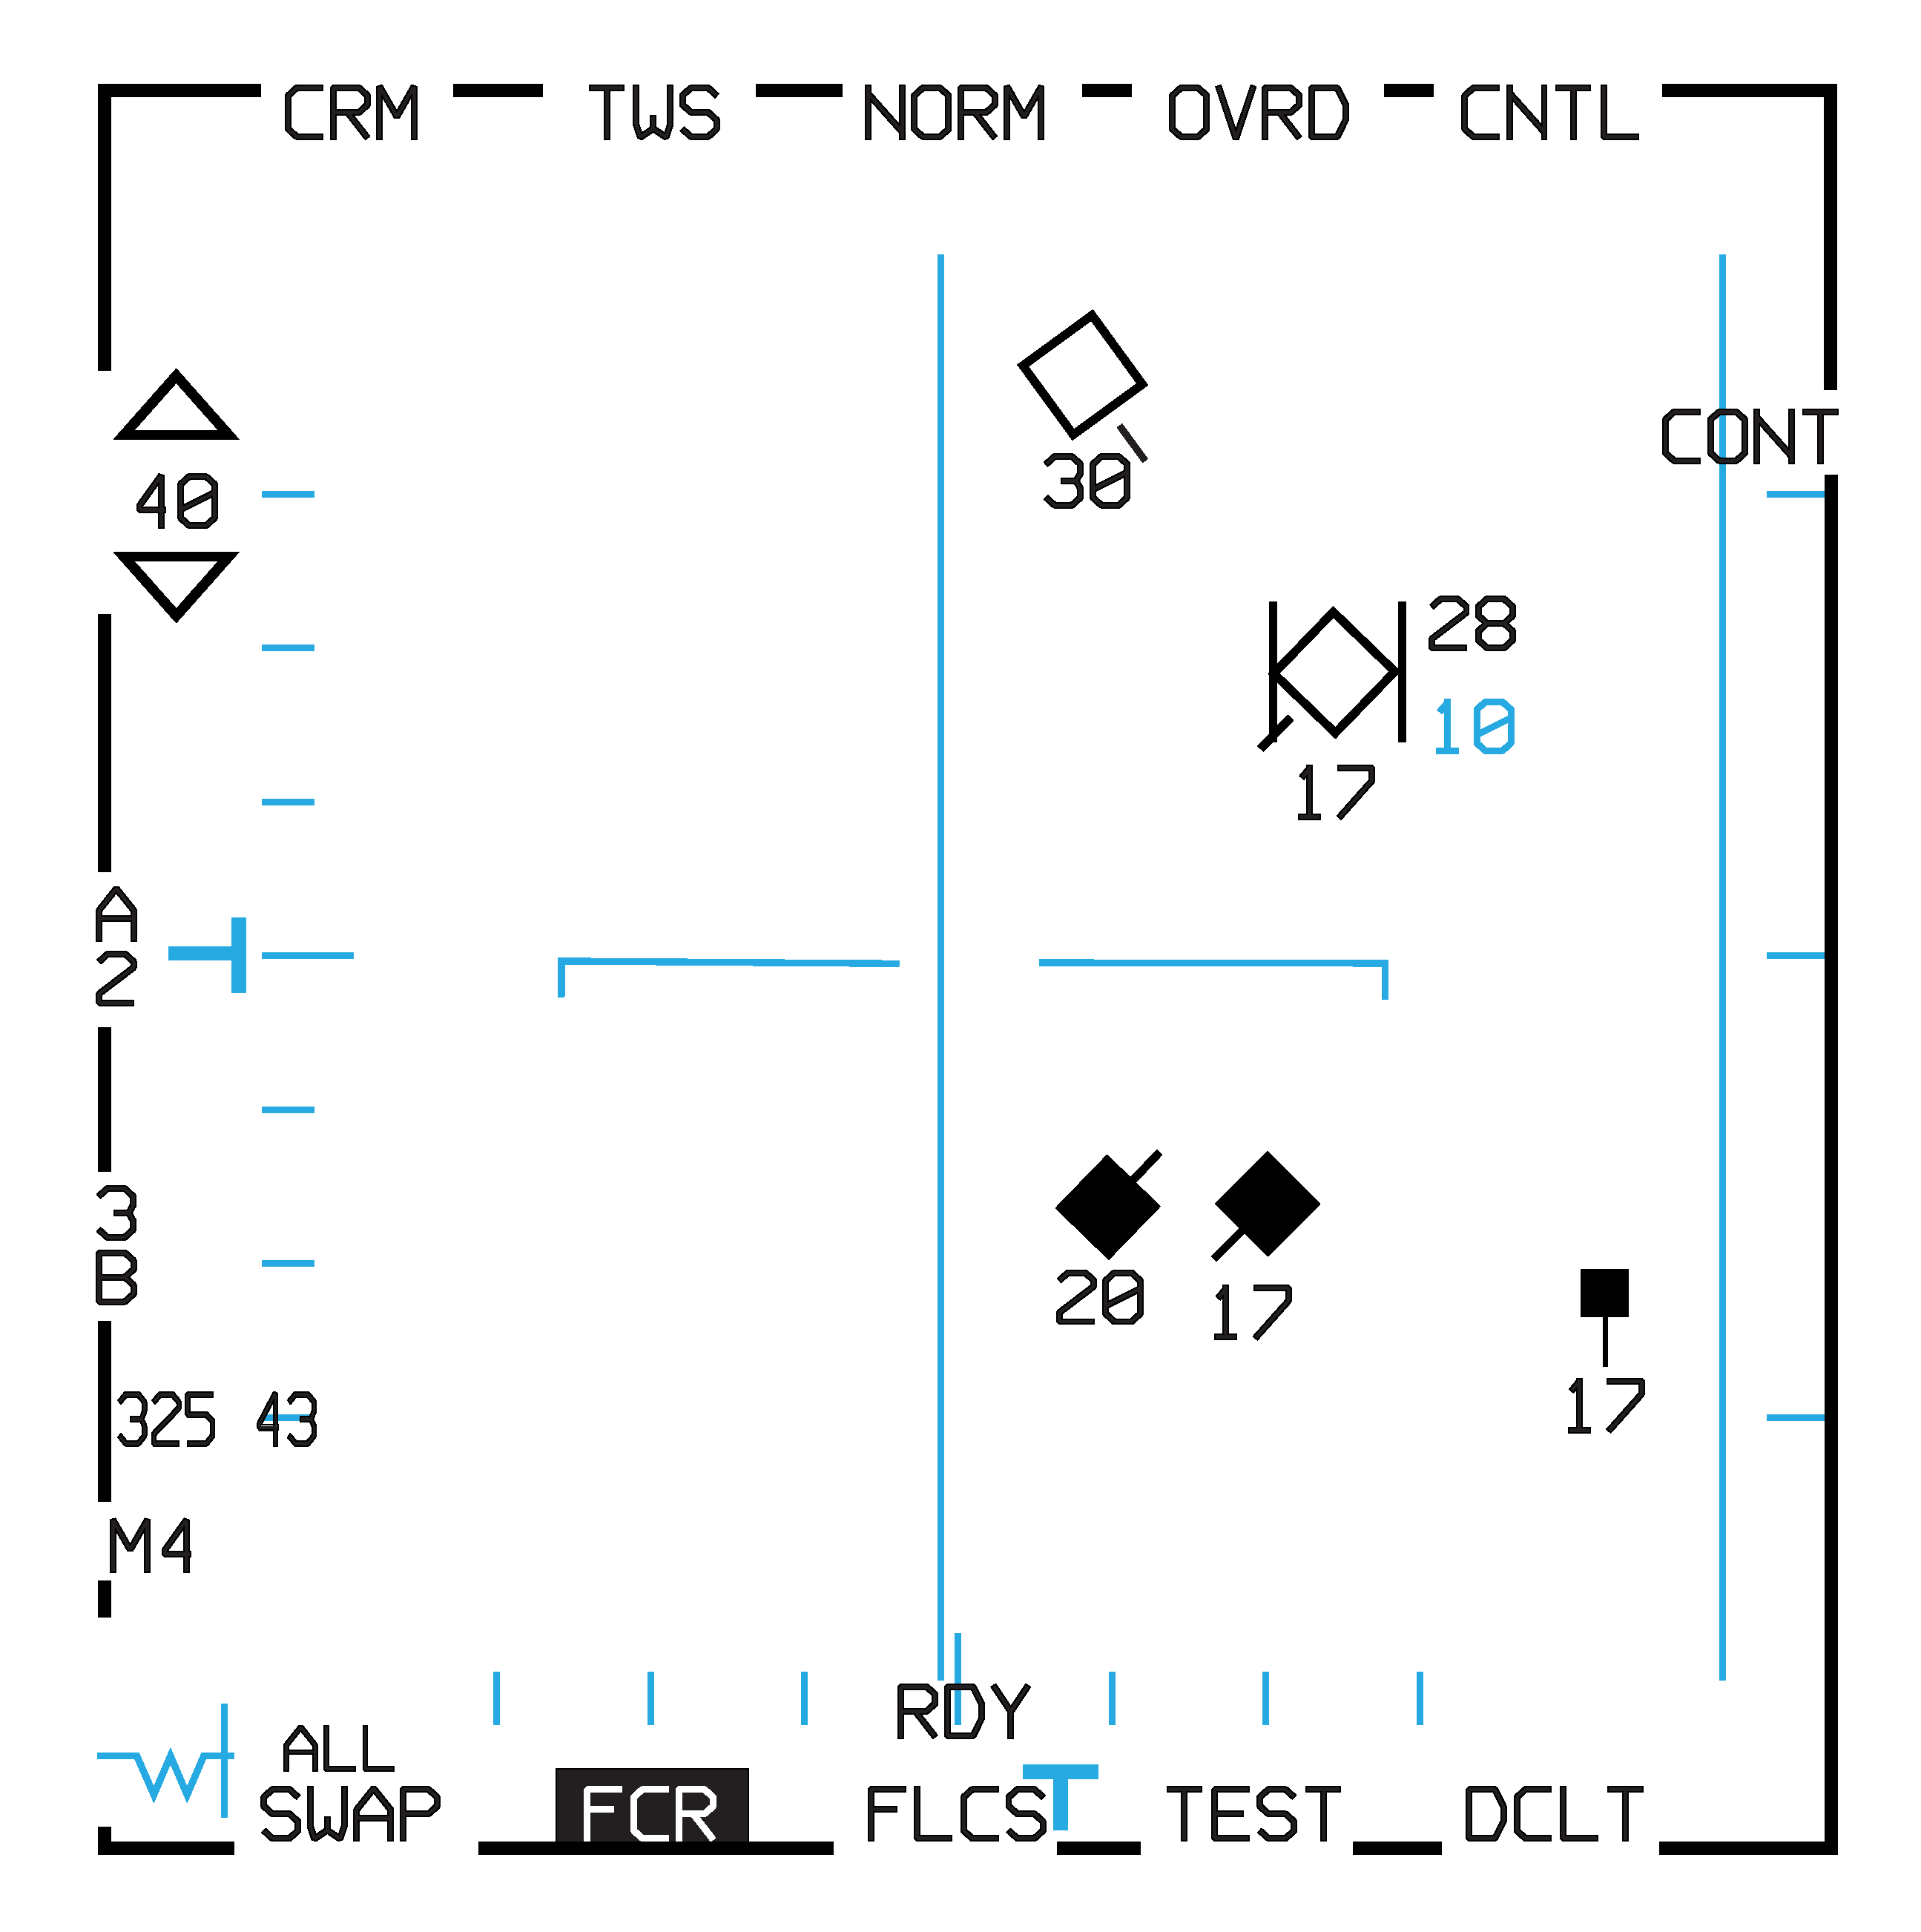
\includegraphics[
                height=75mm,
            ]{mfd/fcr_aa/tws_cursor.pdf}
        };

        % Annotations
        \node[lannot] (system) at ($(fig.west)+(0mm,29mm)$) {System \\ target};
        \draw[->, red] (system.east) -- ++(37mm, 0mm) -- ++(4mm, -4mm);

        \node[lannot] (sec) at ($(fig.west)+(0mm,8mm)$) {Azimuth scan limits};
        \draw[->, red] (sec.east) -- ++(36mm, 0mm);

        \node[rannot] (cursor) at ($(fig.east)+(0mm,11mm)$) {Cursor \\ target};
        \draw[->, red] (cursor.west) -- ++(-15mm, 0mm);

        \node[rannot] (searchr) at ($(fig.east)+(0mm,-15mm)$) {Search \\ target};
        \draw[->, red] (searchr.west) -- ++(-11mm, 0mm);

        \node[rannot] (asec) at ($(fig.east)+(0mm,-26mm)$) {Track \\ targets};
        \draw[->, red] (asec.west) -- ++(-20mm, 0mm) -- ++(-6mm,10mm);
    \end{tikzpicture}
    \caption{TWS FCR page symbology with cursor target}
    \label{fig:sensorsaa:apg68:tws:cursorsymb}
\end{figure}

\begin{figure}[htbp]
    \centering
    \begin{tikzpicture}[auto, node distance=10mm, x=1mm, y=1mm, very thick, line cap=round,
        >={Latex[round]}
        ]
        
        \node[] (mfd) at (0,0) {
            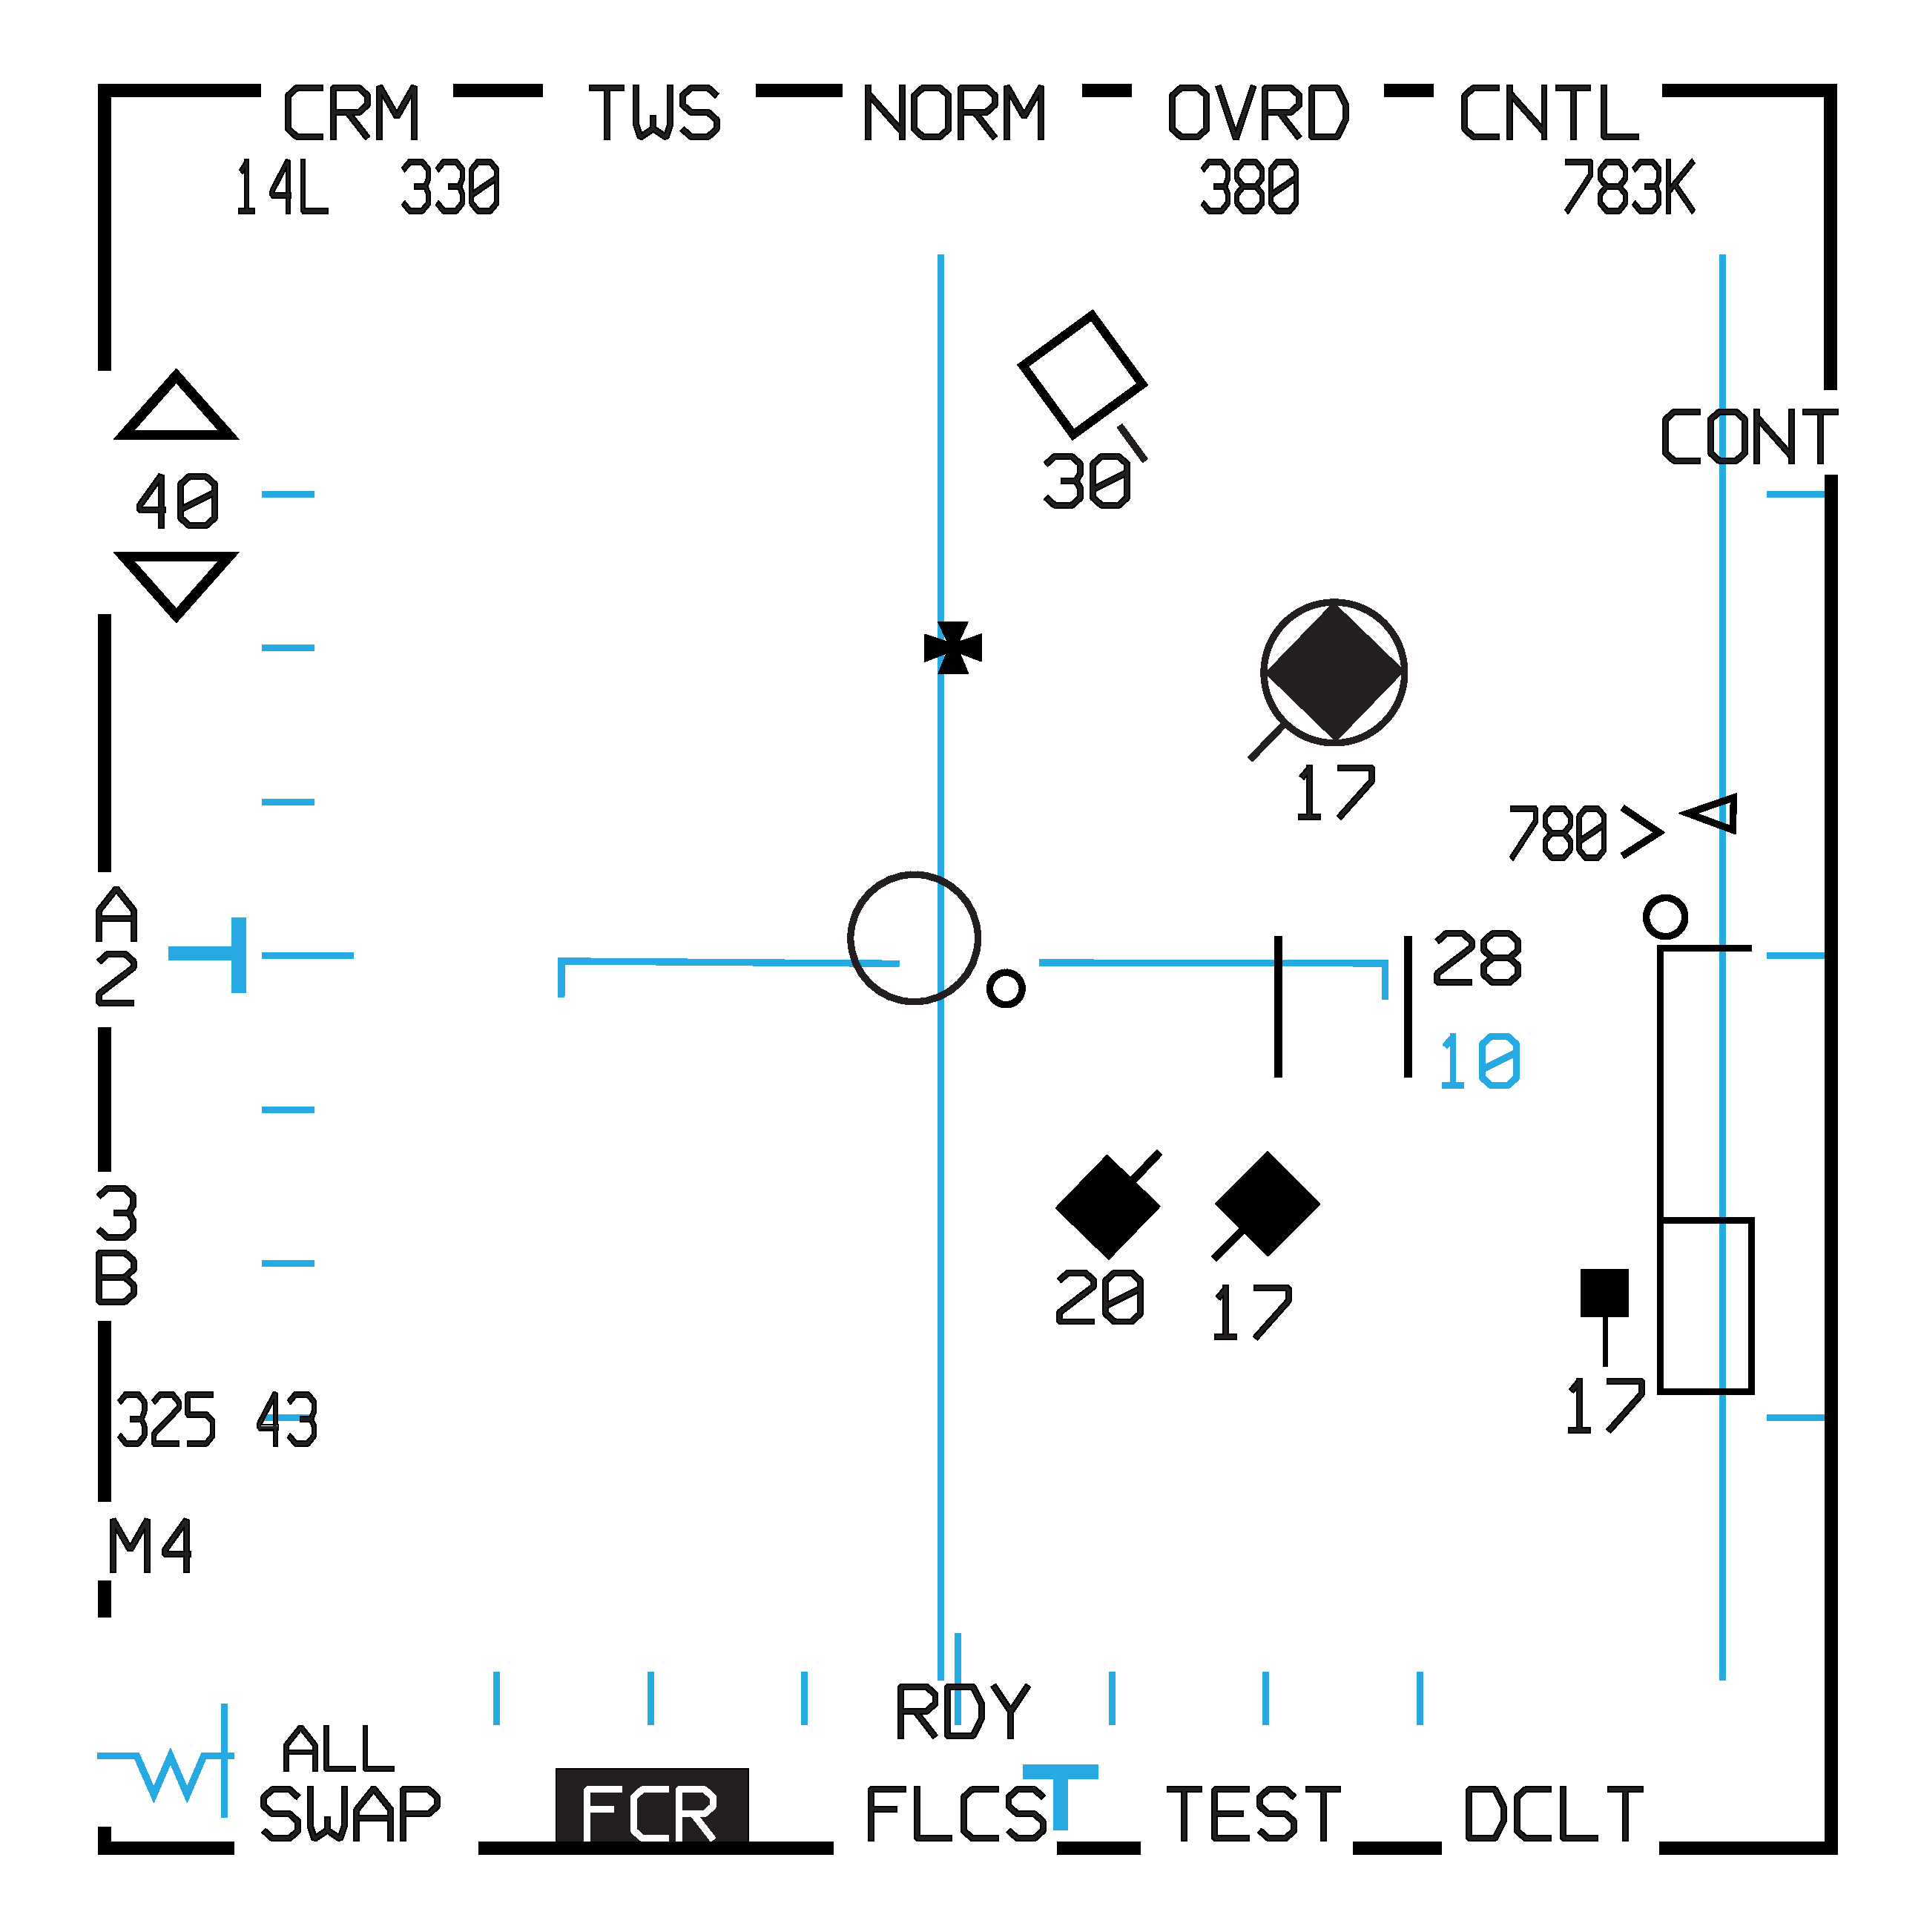
\includegraphics[
                height=75mm,
            ]{mfd/fcr_aa/tws_bugged.pdf}
        };

        % Annotations
        \node[lannot] (asp) at ($(fig.west)+(0mm,30.25mm)$) {Aspect};
        \draw[->, red] (asp.east) -- ++(9mm, 0mm);

        \node[lannot] (trk) at ($(fig.west)+(0mm,24mm)$) {Track};
        \draw[->, red] (trk.east) -- ++(12mm, 0mm) -- ++(4mm, 4mm);

        % \node[lannot] (system) at ($(fig.west)+(0mm,15mm)$) {System \\ target};
        % \draw[->, red] (system.east) -- ++(37mm, 0mm) -- ++(4mm, 4mm);

        \node[lannot] (cross) at ($(fig.west)+(0mm,7mm)$) {Steering \\ cross};
        \draw[->, red] (cross.east) -- ++(32mm, 0mm) -- ++(4mm, 4mm);

        % \node[lannot] (sec) at ($(fig.west)+(0mm,-8mm)$) {Azimuth scan limits};
        % \draw[->, red] (sec.east) -- ++(36mm, 0mm);

        \node[lannot] (asec) at ($(fig.west)+(0mm,-6mm)$) {ASC / ASEC \\ {\footnotesize see \cref{fig:aa_weap:aim120:asc_asec}}};
        \draw[->, red] (asec.east) -- ++(30mm, 0mm) -- ++(4mm, 4mm);

        \node[rannot] (clos) at ($(fig.east)+(0mm,30.25mm)$) {Closure};
        \draw[->, red] (clos.west) -- ++(-9mm, 0mm);

        \node[rannot] (as) at ($(fig.east)+(0mm,24mm)$) {Airspeed};
        \draw[->, red] (as.west) -- ++(-22mm, 0mm) -- ++(-4mm, 4mm);

        \node[rannot] (bug) at ($(fig.east)+(0mm,11mm)$) {Bugged \\ target};
        \draw[->, red] (bug.west) -- ++(-20mm, 0mm);

        \node[rannot] (dlz) at ($(fig.east)+(0mm,-10mm)$) {DLZ \\ {\footnotesize see \cref{fig:aa_weap:aim120:dlz}}};
        \draw[->, red] (dlz.west) -- ++(-7mm, 0mm);

        \node[rannot] (asec) at ($(fig.east)+(0mm,-26mm)$) {Track \\ targets};
        \draw[->, red] (asec.west) -- ++(-20mm, 0mm) -- ++(-6mm,10mm);
    \end{tikzpicture}
    \caption{
        TWS FCR page symbology with bugged target. 
        Note that ``shoot'' symbology (DLZ, ASEC, steering cross) 
        as well as additional information about the bugged target is displayed.
    }
    \label{fig:sensorsaa:apg68:tws:buggedsymb}
\end{figure}

\marginfigeometry

\subsubsection{SELECT TWS MODE}
\begin{checklistenumerate}
    \blueitem{FCR Switch}{\textbf{FCR}}
    \blueitem{Desired MFD}{\textbf{FCR Page}, verify \textbf{SOI}}
    \blueitem{Radar Mode}{
        \textbf{CRM} (default), verify

        \begin{subitemize}
            \item \textbf{Dogfight/Missile Override} --- \textbf{NORM}
            \item \textbf{Radar Mode (OSB 1)} --- shows \textbf{CRM}
        \end{subitemize}
    }
    \blueitem{CRM Submode}{
        \textbf{TWS}, cycle via 

        \begin{subitemize}
            \item \textbf{TMS Right (long)} / \textbf{OSB 2} 
        \end{subitemize}
    }
\end{checklistenumerate}

\subsubsection{MULTI-TARGET ACQUISITION}
\label{subsec:tws:multiacq}
\begin{checklistenumerate}
    \blueitem{Track Target Acquisition}{
    \label{subsec:sensorsaa:apg68:tws:multi:trk}
    \marginpar{
        \captionsetup{type=figure}
        \centering
        \begin{tikzpicture}[figstyle]
            
            \node[
                boxedmarfigstyle,            
            ] (search) at (0,0) {
                
\includegraphics[
                    scale=0.5,
                ]{mfd/fcr_aa/tgt_search.pdf}
            };
            \node[
                boxedmarfigstyle,               
                below=10 of search,
            ] (track) {
                
\includegraphics[
                    scale=0.5,
                ]{mfd/fcr_aa/tgt_track.pdf}
            };
            \node[
                boxedmarfigstyle,
                below=17.5 of track,
            ] (system) {
                
\includegraphics[
                    scale=0.5,
                ]{mfd/fcr_aa/tgt_system.pdf}
            };
            \node[
                boxedmarfigstyle,                
                below=12.5 of system,
            ] (cursor) {
                
\includegraphics[
                    scale=0.5,
                ]{mfd/fcr_aa/tgt_cursor.pdf}
            };
            \node[
                boxedmarfigstyle,                
                below=10 of cursor,
            ] (bugged) {
                
\includegraphics[
                    scale=0.5,
                ]{mfd/fcr_aa/tgt_bugged.pdf}
            };

            % lines
            \draw[->]
            (search) -- node[right, align=left, font=\small] {\textbf{Automatic}}(track);
            \path (search) -- node[left, align=right, font=\small] {\ref{subsec:sensorsaa:apg68:tws:multi:trk}}(track);
            \draw[->]
            (track) -- node[right, align=left, font=\small] {\textbf{TMS FWD} \\ \footnotesize\textbf{(repeat for all} \\ \footnotesize\textbf{desired targets)}}(system);
            \draw[>-]
            ($(track.south)!0.5!(system.north) + (-5,0)$) -- ++(0,2) arc (180:0:2.5) -- ++(0,-4) arc (360:180:2.5) -- node[left, align=right, font=\small, pos=1] {\ref{subsec:sensorsaa:apg68:tws:multi:sys}} ++(0,2);
            \draw[->]
            (system) -- node[right, align=left, font=\small] {\textbf{Slew Cursor} \\ \textbf{near target}}(cursor);
            \draw[->]
            (cursor) -- node[right, align=left, font=\small] {\textbf{TMS FWD}}(bugged);
            \path (cursor) -- node[left, align=right, font=\small] {\ref{subsec:sensorsaa:apg68:tws:multi:bug}}(bugged);

            % labels
            \node[
                anchor=north west,
                align=left,
                font=\bfseries\footnotesize,
            ] (labelsearch) at (search.north west) {Search \\ Target};
            \node[
                anchor=north west,
                align=left,
                font=\bfseries\footnotesize,
            ] (labeltrack) at (track.north west) {Track \\ Target};
            \node[
                anchor=north west,
                align=left,
                font=\bfseries\footnotesize,
            ] (labelsystem) at (system.north west) {System \\ Target};
            \node[
                anchor=north west,
                align=left,
                font=\bfseries\footnotesize,
            ] (labelcursor) at (cursor.north west) {Cursor \\ Target};
            \node[
                anchor=north west,
                align=left,
                font=\bfseries\footnotesize,
            ] (labelbugged) at (bugged.north west) {Bugged \\ Target};
        \end{tikzpicture}
        \caption{TWS trackfile acquisition flow}
    }
    \begin{subenumerate}
        \item Correlate onboard/offboard sensors to locate targets
        \begin{itemize}
            \item raw radar returns, RWR pings
            \item AWACS calls, datalink targets
        \end{itemize}
        \item Place targets within radar scan volume
        \item FCR automatically generates Track Targets once sufficient data available
    \end{subenumerate}}
    \blueitem{System Target Acquisition}{
    \label{subsec:sensorsaa:apg68:tws:multi:sys}
    \begin{subenumerate}
        \item \textbf{Target} \dotfill under Acquisition Cursor
        \item \textbf{TMS} \dotfill \textbf{Forward} 
    \end{subenumerate}
    Repeat for all desired Track Targets,
    or to upgrade all Track Targets:
    \begin{subenumerate}
        \item \textbf{TMS} \dotfill \textbf{Right}
    \end{subenumerate}}
    \blueitem{Upgrade to Bugged Target}{
    \label{subsec:sensorsaa:apg68:tws:multi:bug}
    \begin{subenumerate}
        \item \textbf{Target} \dotfill under Acquisition Cursor
        \item \textbf{TMS} \dotfill \textbf{Forward}
    \end{subenumerate}
    To select closest System Target 
    \begin{subenumerate}
        \item \textbf{TMS} \dotfill \textbf{Right}
    \end{subenumerate}
    To cycle through System Targets in range order
    \begin{subenumerate}
        \item \textbf{TMS} \dotfill \textbf{Right}
    \end{subenumerate}}
    \blueitem{STT Lock}{(if desired)
    \begin{subenumerate}
        \item \textbf{Bugged Target} \dotfill under Acq Cursor
        \item \textbf{TMS} \dotfill \textbf{Forward}
    \end{subenumerate}}
\end{checklistenumerate}

\marginfigrestore